\chapter{Datové struktury a algoritmy}


\section{B-tree}

B-tree\cite{Cormen:2001:IA:580470} je zobecněný binární strom s~možností
mít více jak 2 potomky. Jeho optimalizován pro čtení a zápis velkého
objemu dat, takže je se hojně používá v~databázích a souborových
systémech.

\begin{figure}[t]
\centering{}\caption{B-tree}
\end{figure}



\subsection{Definice}

B-tree $T$ je kořenový strom (s~kořenem $root[T]$) s~následujícími
vlastnostmi:
\begin{enumerate}
\item Každý uzel $x$ obsahuje následující prvky:

\begin{enumerate}
\item $n[x]$ - počet klíčů uložených v~uzlu $x$,
\item $n[x]$ samotných klíčů, uložených v~neklesajícím pořadí, tedy \linebreak $key_{1}[x]\leq key_{2}[x]\leq\cdots\leq key_{n[x]}[x]$,
\item $leaf[x]$ typu boolean, který je TRUE pokud $x$ je list a FALSE
pokud je $x$ interní uzel\@.
\end{enumerate}
\item Každý vnitřní uzel $x$ obsahuje $n[x]+1$ ukazatelů
\footnote{v~případě jazyka Java \emph{referencí}
} $c_{1}[x],c_{2}[x],\ldots{},c_{n[x]+1}[x]$ na jeho potomky (\emph{children}).
Uzly listů nemají žádné potomky -- jejich $c_{i}$ prvky jsou nedefinovány.
\item Klíče $key_{i}[x]$ oddělují rozsahy klíčů uložených v~každém podstromu:
pokud $k_{i}$ je libovolný klíč uložený v~podstromu s~kořenem $c_{i}[x]$,
pak
\[
k_{1}\leq key_{1}[x]\leq k_{2}\leq key_{2}[x]\leq\cdots\leq key_{n[x]}[x]\leq k_{n[x]+1}.
\]

\item Všechny listy mají stejnou hloubku, která se nazývá výška stromu $h$\@.
\item Jsou definovány spodní a horní hranice na množství klíčů, které může
uzel obsahovat\@. Tyto hranice můžou být vyjádřeny pomocí fixního
čísla $t\geq2$ zvaného \emph{minimální stupeň} B-tree:

\begin{enumerate}
\item Každý uzel jiný než kořen musí mít alespoň $t-1$ klíčů.
Každý interní uzel jiný než kořen má alespoň $t$ potomků.
Pokud není strom prázdný, potom kořen má alespoň jeden klíč.
\item Každý uzel obsahuje nejvýše $2t-1$ klíčů.
Proto interní uzel může mít nejvýše $2t$ potomků.
Řekneme, že uzel je plný, pokud obsahuje přesně $2t-1$ klíčů.
\end{enumerate}
\end{enumerate}

\subsection{Asymptotická složitost}
\begin{center}
\begin{tabular}{|c|c|}
\hline 
Operace & Asymptotická složitost\tabularnewline
\hline 
\hline 
SEARCH & \BigO{\log n} \\
\hline 
INSERT & \BigO{\log n} \\
\hline 
DELETE & \BigO{\log n} \\
\hline 
\end{tabular}
\end{center}

\subsection{Prohledávání B-tree (B-Tree-Search)}

Prohledávání B-tree je velmi podobné jako prohledávání binárního stromu\@.
Pouze místo binárního větvení v~každém uzlu, se provádí vícecestné
větvení podle počtu potomků uzlu\@.

Vstupem je ukazatel na kořenový uzel podstromu $x$ a klíč $k$, který
má být prohledán v~podstromu\@. První volání je tedy B-Tree-Search($root[T],k$).
Pokud je $k$ v~B-tree, pak vyhledávání vrátí uspořádanou dvojici
$(y,i)$, kde $y$ je ukazatel na uzel a $i$ je pozice, takže $key_{i}[y]=k$\@.
Jinak je vrácena \uv{prázdná} dvojice.
\footnote{Původně je v~\cite{Cormen:2001:IA:580470} NIL, jenže obecně vracení
NIL, NULL a 0 ukazatelů/referencí komplikuje pozdější práci s~návratovou
hodnotou metody. Robert~C.~Martin doporučuje místo prázdné
reference, vracet \uv{prázdný} objekt\cite{martin2009clean}.
V~praxi často dochází ke zneužívání návratové hodnoty v~podobě
\type{NULL}, jako dalšího stavu. Místo předpokladu na existující objekt,
je nutno dělat kontrolu na neexistující objekt. Jaký je rozdíl mezi
vrácením prázdné kolekce/kontejneru nebo nulového ukazatele?
}

\begin{algorithm}[t]
\SetAlgoLined
\SetKwData{EMPTYTUPLE}{EMPTY\_TUPLE}
\SetKwFunction{BTreeSearch}{B-Tree-Search}
\SetKw{KwAnd}{and}

$i \longleftarrow 1$\\
\While{$i \leq n[x]$ \KwAnd $k \le key_i[x]$}{
	$i \longleftarrow i+1$}
\If{$i \leq n[x]$ \KwAnd $k = key_i[x]$}{
	\Return{x, i}}
\eIf{leaf[x]}{
	\Return{\EMPTYTUPLE}}{
        \Return{\BTreeSearch{$c_i[x], k$}}}

\caption{B-Tree-Search($x,k$)}
\end{algorithm}



\subsection{Operace INSERT}

Vkládání do B-tree je výrazně složitější než stejná operace pro binární strom.
Podobně jako u~binárního stromu hledáme pozici listu kde uložíme klíč.
Bohužel u~B-tree nemůžeme jednoduše vytvořit nový uzel pro list a ten vložit, protože výsledný strom by nebyl validní B-tree.
Místo toho se vloží klíč do už existujícího listu.
Protože nelze vložit klíč do plného listu, zavedeme operaci rozdělení (\emph{split}) plného uzlu $y$ (s~$2t-1$ klíči) okolo svého \emph{mediánu klíčů} $key_{t}[y]$ na dva uzly, z~nichž každý má $t-1$ klíčů.
\emph{Medián klíč} se přesune do rodiče $y$ k~identifikaci dělícího bodu mezi dvěma novými stromy.
Pokud je rodič $y$ také plný, musí být nejdříve rozdělen před vložením nového klíče.
Dělení plných uzlů se může tedy propagovat celým stromem nahoru.

\subsubsection{Rozdělení uzlu v~B-tree}

Vstupem pro proceduru B-Tree-Split-Child je neplný vnitřní uzel $x$,
index $i$ a uzel $y$, tak že $y=c_{i}[x]$ je plným potomkem $x$\@.
Procedura poté rozdělí potomka na dva a upraví $x$ tak, že má dalšího
potomka.

Složitost je \BigO{t}.

%\begin{figure}[t]
%\caption{Rozdělení (\emph{split}) uzlu}
%\end{figure}
%

\begin{algorithm}[t]
\SetAlgoLined
\SetKwFunction{BTreeSplitChild}{B-Tree-Split-Child}
\SetKwFunction{AllocateNode}{Allocate-Node}
\SetKw{Not}{not}
\SetKw{KwDownto}{downto}

{$z \longleftarrow \AllocateNode$}\\
{$leaf[z] \longleftarrow leaf[y]$}\\
{$n[z] \longleftarrow t-1$}\\
\For{ $j \longleftarrow 1$ \KwTo $t-1$}{
	$key_j[z] \longleftarrow key_{(j+t)}[y]$}
\If{ \Not $leaf[y]$}{
	\For{$j \longleftarrow 1$ \KwTo $t$}{
		$c_j[z] \longleftarrow c_{(j+t)}[y]$}
}
$n[y] \longleftarrow t-1$\\
\For{$j \longleftarrow n[x]+1$ \KwDownto $i+1$}{
	$c_{(j+1)}[x] \longleftarrow c_j[x]$}
$c_{(i+1)}[x] \longleftarrow z$\\
\For{$j \longleftarrow n[x]$ \KwDownto $i$}{
	$key_{(j+1)}[x] \longleftarrow key_j[x]$}
$key_i[x] \longleftarrow key_t[y]$\\
$n[x] \longleftarrow n[x]+1$
\caption{B-Tree-Split-Child($x, i, y$)}
\end{algorithm}



\subsubsection{Vložení klíčů do B-tree jedním průchodem stromem}

K~vložení klíče $k$ do B-tree $T$ o~výšce $h$ jedním průchodem
potřebujeme $O(th)=O(t\log_{t}n)$\@. B-Tree-Insert používá B-Tree-Split-Child
k~zajištění toho, že rekurse nikdy nedojde k~plnému uzlu\@.

\begin{algorithm}[t]
\SetAlgoLined
\SetKwFunction{BTreeInsert}{B-Tree-Insert}
\SetKwFunction{BTreeSplitChild}{B-Tree-Split-Child}
\SetKwFunction{BTreeInsertNonfull}{B-Tree-Insert-Nonfull}
\SetKwFunction{AllocateNode}{Allocate-Node}
\SetKw{FALSE}{FALSE}

$r\longleftarrow root[T]$
\eIf{$n[r] = 2t-1$}{
	$s \longleftarrow \AllocateNode$\\
		$root[T] \longleftarrow s$\\
		$leaf[s] \longleftarrow \FALSE$\\
		$n[s] \longleftarrow 0$\\
		$c_1[s] \longleftarrow r$\\
		\BTreeSplitChild{s, 1, r}\\
		\BTreeInsertNonfull{s,k}
}{\BTreeInsertNonfull{r,k}}

\caption{B-Tree-Insert($T,k$)}
\end{algorithm}

Procedura B-Tree-Insert-Nonfull se vnořuje podle potřeby do stromu, přičemž v~každém okamžiku garantuje, že uzel do kterého se vnořila, není plný díky volání B-Tree-Split-Child.

Rekursivní procedura B-Tree-Insert-Nonfull vloží klíč $k$ do uzlu $x$, který je předpokládán neplný v~okamžiku volání procedury.
Díky B-Tree-Insert a rekursivní B-Tree-Insert-Nonfull je tento předpoklad zajištěn.

\begin{algorithm}[t]
\SetAlgoLined
\SetKwFunction{BTreeSplitChild}{B-Tree-Split-Child}
\SetKwFunction{BTreeInsertNonfull}{B-Tree-Insert-Nonfull}
\SetKw{KwAnd}{and}

$i \longleftarrow n[x]$\\
\eIf{leaf[x]}{
	\While{$i >= 1$ \KwAnd $k < key_i[x]$}{
			$key_{(i+1)}[x] \longleftarrow key_i[x]$\\
				$i \longleftarrow i-1$}
		$key_{(i+1)}[x] \longleftarrow k$\\
		$n[x] \longleftarrow n[x]+1$
}{\While{$i >= 1$ \KwAnd $k < key_i[x]$}{
			$i \longleftarrow i-1$}
		$i \longleftarrow i+1$\\
		\If{$n[c_i[x]] \longleftarrow 2t-1$}{
			\BTreeSplitChild{x,i,$c_i[x]$}\\
				\If{$k > key_i[x]$}{
					$i \longleftarrow i+1$}
}

\BTreeInsertNonfull{$c_i[x]$,k}
}

\caption{B-Tree-Insert-Nonfull($x,k$)}
\end{algorithm}

\subsection{Operace DELETE}

Není nutná pro potřeby této práce a její popis je vynechán.
Detailní popis je možné najít v~\cite{Cormen:2001:IA:580470}.


\section{\BPTree\label{sec:B-plus-tree}}

\BPTree{} je varianta B-tree, která ukládá hodnoty až do
listů stromu. Do interních uzlů ukládá pouze informace o~klíčích
a ukazatelích na potomky. Každý koncový uzel udržuje ukazatel na další
koncový uzel. To umožňuje velmi elegantně vytvořit vyhledávání v~rozsahu.

Tento typ maximalizuje větvení interních uzlů.

Je použit v~souborových systémech, např. NTFS \cite{Carrier:2005:FSF:1051914}, btrfs, ZFS \cite{Powell:2012:ZBQ:2328941.2328946} atd\ldots{}
Dále v~databázích PostgreSQL \cite{Geschwinde:2001:PDH:580250}, Oracle \cite{Kyte:2003:EOD:1593880} atd\ldots{}


\begin{figure}[ht]
\center
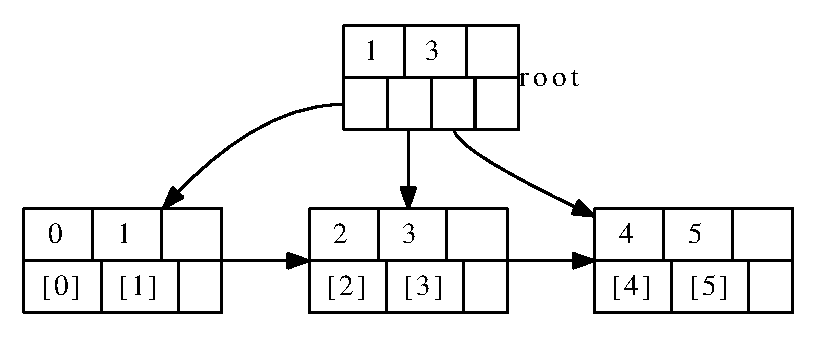
\includegraphics{bptree}
\caption{\BPTree}
\end{figure}

\subsection{Asymptotická složitost}
Pro \BPTree{} se stupněm $t$ a počtem klíčů $n$ platí:
\begin{center}
\begin{tabular}{|p{4cm}|c|}
\hline 
Operace & Asymptotická složitost \\
\hline 
\hline 
SEARCH & \BigO{\log_b n} \\
\hline 
SEARCH pro rozsah ($k$ je počet prvků nacházejících se v dotazu) & $\mathcal{O}(\log_b n + k)$ \\
\hline 
INSERT & \BigO{\log_b n} \\
\hline 
DELETE & \BigO{\log_b n} \\
\hline 
\end{tabular}
\end{center}

\section{Voroného diagram}
Voroného diagram je rozdělení prostoru na oblasti, které obsahují k~sobě nejbližší body\cite{dorst2010geometric}.

\begin{figure}[ht]
\center
\includegraphics[width=0.5\textwidth]{voronoi}
\caption{Voroného diagram\cite{wiki:voronoidiagram}}
\end{figure}
